%%%%%%%%%%%%%%%%%%%%%%%%%%%%%%%%%%%%%%%%%
% Programming/Coding Assignment
% LaTeX Template
%
% This template has been downloaded from:
% http://www.latextemplates.com
%
% Original author:
% Ted Pavlic (http://www.tedpavlic.com)
%
% Note:
% The \lipsum[#] commands throughout this template generate dummy text
% to fill the template out. These commands should all be removed when 
% writing assignment content.
%
% This template uses a Perl script as an example snippet of code, most other
% languages are also usable. Configure them in the "CODE INCLUSION 
% CONFIGURATION" section.
%
%%%%%%%%%%%%%%%%%%%%%%%%%%%%%%%%%%%%%%%%%

%----------------------------------------------------------------------------------------
%	PACKAGES AND OTHER DOCUMENT CONFIGURATIONS
%----------------------------------------------------------------------------------------

\documentclass{article}

\usepackage{fancyhdr} % Required for custom headers
\usepackage{lastpage} % Required to determine the last page for the footer
\usepackage{extramarks} % Required for headers and footers
\usepackage[usenames,dvipsnames]{color} % Required for custom colors
\usepackage{graphicx} % Required to insert images
\usepackage{listings} % Required for insertion of code
\usepackage{courier} % Required for the courier font
\usepackage{lipsum} % Used for inserting dummy 'Lorem ipsum' text into the template
\usepackage{url}

\usepackage{hyperref}

% Margins
\topmargin=-0.45in
\evensidemargin=0in
\oddsidemargin=0in
\textwidth=6.5in
\textheight=9.0in
\headsep=0.25in

\linespread{1.1} % Line spacing

% Set up the header and footer
\pagestyle{fancy}
\lhead{\hmwkAuthorName} % Top left header
\chead{\hmwkClass\ (\hmwkClassInstructor\ \hmwkClassTime)} % Top center head
\rhead{\firstxmark} % Top right header
\lfoot{\lastxmark} % Bottom left footer
\cfoot{} % Bottom center footer
\rfoot{Page\ \thepage\ of\ \protect\pageref{LastPage}} % Bottom right footer
\renewcommand\headrulewidth{0.3pt} % Size of the header rule
\renewcommand\footrulewidth{0.4pt} % Size of the footer rule

\setlength\parindent{0pt} % Removes all indentation from paragraphs



%----------------------------------------------------------------------------------------
%	CODE INCLUSION CONFIGURATION
%----------------------------------------------------------------------------------------

\definecolor{MyDarkGreen}{rgb}{0.0,0.4,0.0} % This is the color used for comments
\lstloadlanguages{R} % Load Perl syntax for listings, for a list of other languages supported see: ftp://ftp.tex.ac.uk/tex-archive/macros/latex/contrib/listings/listings.pdf
\lstset{language=R, % Use Perl in this example
        frame=single, % Single frame around code
        basicstyle=\small\ttfamily, % Use small true type font
        breaklines=true,
        keywordstyle=[1]\color{Blue}\bf, % Perl functions bold and blue
        keywordstyle=[2]\color{Purple}, % Perl function arguments purple
        keywordstyle=[3]\color{Blue}\underbar, % Custom functions underlined and blue
        identifierstyle=, % Nothing special about identifiers                                         
        commentstyle=\usefont{T1}{pcr}{m}{sl}\color{MyDarkGreen}\small, % Comments small dark green courier font
        stringstyle=\color{Purple}, % Strings are purple
        showstringspaces=false, % Don't put marks in string spaces
        tabsize=5, % 5 spaces per tab
        %
        % Put standard Perl functions not included in the default language here
        morekeywords={},
        %
        % Put Perl function parameters here
        morekeywords=[2]{on, off, interp},
        %
        % Put user defined functions here
        morekeywords=[3]{test},
       	%
        morecomment=[l][\color{Blue}]{...}, % Line continuation (...) like blue comment
        numbers=left, % Line numbers on left
        firstnumber=1, % Line numbers start with line 1
        numberstyle=\tiny\color{Blue}, % Line numbers are blue and small
        stepnumber=5 % Line numbers go in steps of 5
}

% Creates a new command to include a perl script, the first parameter is the filename of the script (without .pl), the second parameter is the caption
\newcommand{\rscript}[2]{
\begin{itemize}
\item[]\lstinputlisting[caption=#2,label=#1]{#1.R}
\end{itemize}
}

%----------------------------------------------------------------------------------------
%	DOCUMENT STRUCTURE COMMANDS
%	Skip this unless you know what you're doing
%----------------------------------------------------------------------------------------

% Header and footer for when a page split occurs within a problem environment
\newcommand{\enterProblemHeader}[1]{
\nobreak\extramarks{#1}{#1 continued on next page\ldots}\nobreak
\nobreak\extramarks{#1 (continued)}{#1 continued on next page\ldots}\nobreak
}

% Header and footer for when a page split occurs between problem environments
\newcommand{\exitProblemHeader}[1]{
\nobreak\extramarks{#1 (continued)}{#1 continued on next page\ldots}\nobreak
\nobreak\extramarks{#1}{}\nobreak
}

\setcounter{secnumdepth}{0} % Removes default section numbers
\newcounter{homeworkProblemCounter} % Creates a counter to keep track of the number of problems

\newcommand{\homeworkProblemName}{}
\newenvironment{homeworkProblem}[1][Problem \arabic{homeworkProblemCounter}]{ % Makes a new environment called homeworkProblem which takes 1 argument (custom name) but the default is "Problem #"
\stepcounter{homeworkProblemCounter} % Increase counter for number of problems
\renewcommand{\homeworkProblemName}{#1} % Assign \homeworkProblemName the name of the problem
\section{\homeworkProblemName} % Make a section in the document with the custom problem count
\enterProblemHeader{\homeworkProblemName} % Header and footer within the environment
}{
\exitProblemHeader{\homeworkProblemName} % Header and footer after the environment
}

\newcommand{\problemAnswer}[1]{ % Defines the problem answer command with the content as the only argument
\noindent\framebox[\columnwidth][c]{\begin{minipage}{0.98\columnwidth}#1\end{minipage}} % Makes the box around the problem answer and puts the content inside
}

\newcommand{\homeworkSectionName}{}
\newenvironment{homeworkSection}[1]{ % New environment for sections within homework problems, takes 1 argument - the name of the section
\renewcommand{\homeworkSectionName}{#1} % Assign \homeworkSectionName to the name of the section from the environment argument
\subsection{\homeworkSectionName} % Make a subsection with the custom name of the subsection
\enterProblemHeader{\homeworkProblemName\ [\homeworkSectionName]} % Header and footer within the environment
}{
\enterProblemHeader{\homeworkProblemName} % Header and footer after the environment
}

\newcommand{\quotes}[1]{``#1''}
%----------------------------------------------------------------------------------------
%	NAME AND CLASS SECTION
%----------------------------------------------------------------------------------------

\newcommand{\hmwkTitle}{Homework\ \#6} % Assignment title
\newcommand{\hmwkDueDate}{November 12} % Due date
\newcommand{\hmwkClass}{Applied Data Mining} % Course/class
\newcommand{\hmwkClassTime}{Online} % Class/lecture time
\newcommand{\hmwkClassInstructor}{Instructor: Hasan Kurban} % Teacher/lecturer
\newcommand{\hmwkAuthorName}{Keith Hickman} % Your name

%----------------------------------------------------------------------------------------
%	TITLE PAGE
%----------------------------------------------------------------------------------------

\title{
\vspace{2in}
\textmd{\textbf{\hmwkClass:\ \hmwkTitle}}\\
\normalsize\vspace{0.1in}\small{Due\ on\ \hmwkDueDate}\\
\vspace{0.1in}\large{\textit{\hmwkClassInstructor\ }}
\vspace{3in}
}

\author{\textbf{\hmwkAuthorName}}
\date{\today} % Insert date here if you want it to appear below your name

%----------------------------------------------------------------------------------------

\begin{document}

\maketitle

%----------------------------------------------------------------------------------------
%	TABLE OF CONTENTS
%----------------------------------------------------------------------------------------

%\setcounter{tocdepth}{1} % Uncomment this line if you don't want subsections listed in the ToC

%\newpage
%\tableofcontents
\newpage

%%%%%%%%%%%%%%%%%%%%%%%%%%%%%%%%%%
In this homework, you will work on some of basic tasks of data mining: data preprocessing, exploratory
data analysis and predictive model construction. Fit a linear regression model to the house prices data.
Use “train.csv” and “test.csv” data sets for training and testing purposes, respectively. [150 pt]

Optional: In addition to training a linear regression model, you are encouraged to use other techniques/algorithms
to design a better predictive model.


 
%%%%%%%%%%%%%%%%%%%%%%%%%%%%%%%%%%

%PROBLEM 1
%%%%%%%%%%%%%%%%%%%%%%%%%%%%%%%%%%
\begin{homeworkProblem}
I found a kernel from Kaggle User AiO at:  https://www.kaggle.com/notaapple/detailed-exploratory-data-analysis-using-r
that has some interesting exploratory techniques that I will reproduce here. 
\subsection{R Code}
\rscript{sb1}
\rscript{sb2}{Sample R Script With Highlighting}

\end{homeworkProblem}


%%%%%%%%%%%%%%%%%%%%%%%%%%%%%%%%%

%PROBLEM 2
%%%%%%%%%%%%%%%%%%%%%%%%%%%%%%%%%%
\begin{homeworkProblem}

\subsection{Data Visualization and Summarization  [50 pt]}

\begin{enumerate} 
\item Observe the statistical properties of the data using \quotes{summary} function and briefly discuss each variable.
   \subsection{Discussion of Variables}
The first two variables, MPG and Cylinders appear to be actually discrete, as they take on only a few numeric values.  We can treat these as categories later on.  The next four variables displacement, horsepower, weight, and acceleration are continuous.  MPG, which is likely the target variable, is non-normally distributed and slightly right-skewed.  Other variables are either normal, roughly normal, or non-normal and slightly skewed to the right.  
 I decided to drop the last two variables, as they were mostly missing, they likely wouldn't add any predictive value, and if they added any analytic or descriptive value, we could add them back in after the fact.  \ldots
     
 \item  Create a histogram and Q-Q plot of variable \quotes{displacement}. Using the plots, explain whether or not variable  \quotes{displacement} follows a normal distribution. Discuss the plots (Use ggplot2 and car  packages  to make histogram and Q-Q plot figures). 
 
 \subsection{R Code}

\subsection{Histogram and Q-Q plot Figures}

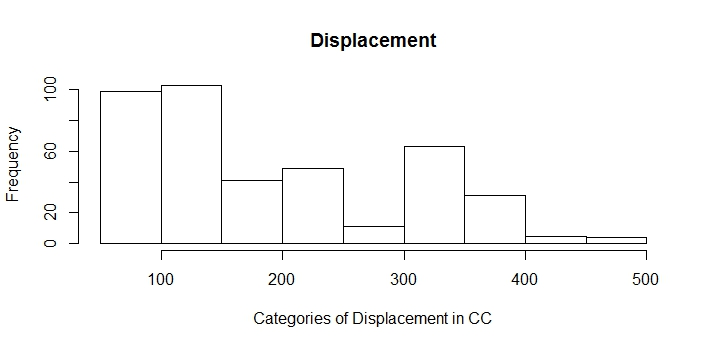
\includegraphics{displacement_hist.jpeg}
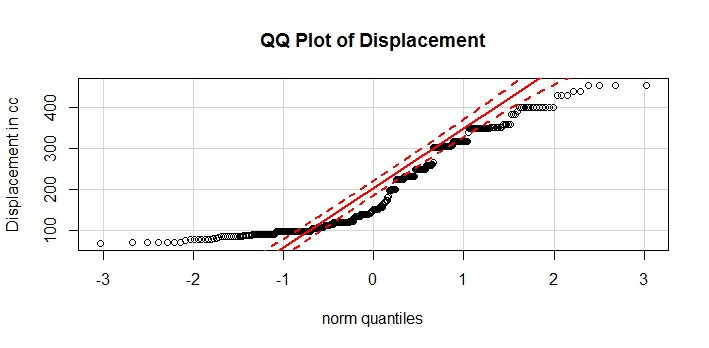
\includegraphics{displacement_qq.jpeg}
 
    \subsection{Discussion of Plots}
        The distribution of the displacement variable is clearly non-normal, as evidenced by both the QQ plot and the Histogram.  According to the Histogram, the distribution is right-skewed, with most values falling in the 75-200 range, with another cluster of values at the 300 range.  The QQ plot shows that there are quite a few values at the tail ends of the distribution.  
        
 \item Box plots provide some key properties of a continuous variable. Create a box plot of variable \quotes{weight} and discuss the the distribution of values, i.e., skewed.  Discuss variable \quotes{weight} using the box plot (Use ggplot2 package).
 
 \subsection{R Code}

\rscript{sb3}{Sample R Script With Highlighting}

\subsection{Box plot Figure}

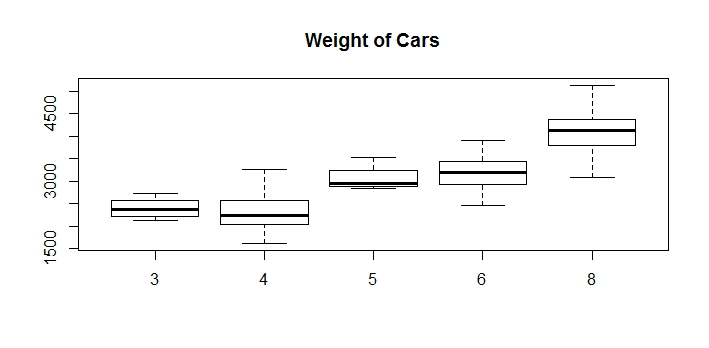
\includegraphics{weight_boxes.jpeg}
 
    \subsection{Discussion of Plots}

The weights variable is a non-normal distribution and is right-skewed, indicating that most of the values fall into categories of cars that weigh less than 3500 pounds.  Additionally, there don't appear to be any outliers.  An examination of the boxplots comparing the weight variable across (the randomly-selected variable) the cylinder variable indicates that the cars which are 4, 6, or 8 cylinders are normally distributed, while cars that have either 3 or 5 cylinders are right skewed and non-normal.     \ldots          
        
 \item Make a set of box plots (conditional box plot) to observe how the distribution of \quotes{mpg} variable looks with the \quotes{origin} variable. Do not forget to convert the \quotes{origin} variable to a factor variable. In additional to the box plot, create a violin plot  of \quotes{mpg} variable against \quotes{origin} variable. Discuss the plots.
\begin{verbatim}
data[,8] < - as.factor(data[,8])
\end{verbatim} 

Similarly, you should also convert other categorical variables into factor variables (Variables 2 and 7).

 \subsection{R Code}

\rscript{sb4}{Sample R Script With Highlighting}

\subsection{Figures}

 Place the figures here.
 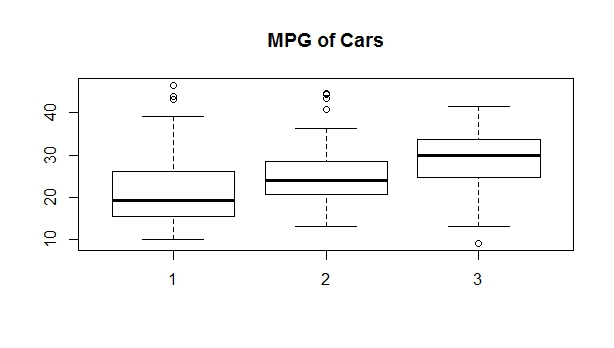
\includegraphics{p4_mpgboxplot.jpeg}
 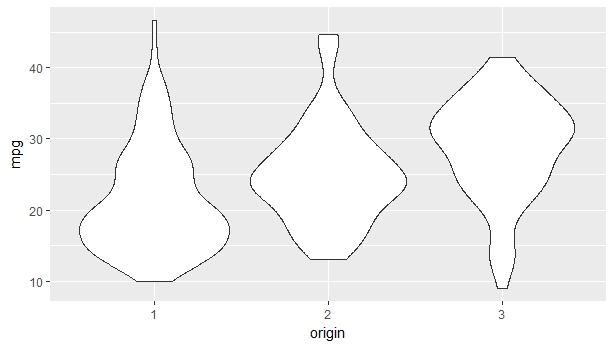
\includegraphics{p4_mpgviolin.jpeg}
 

    \subsection{Discussion of Plots}
        The boxplot and violin plots illustrate a likely correlation between origin and mpg - cars made in the US tend to have an mpg beween 15-25 with a mean slightly below 20. Cars made in Europe (2) are clustered at 25-30, and cars made in Japan tend to have the highest mpg ratings at 30+.  Both plots provide similar information about distribution, however the boxplot also indicates that the distribution of US-made is more spread out, and includes some outliers which we need to investigate.Surprisingly, two of the top four highest-rated mpg cars are US-made.    \ldots 
        
  \item Discretize  \quotes{weight} variable as shown in the textbook, page $203$. Observe  the behavior of  variable "mpg"  conditioned by \quotes{weight} and \quotes{origin} variables over a conditional plot. Discuss the plot.

 \subsection{R Code}

\rscript{sb5}{Sample R Script With Highlighting}

\subsection{Figure}

 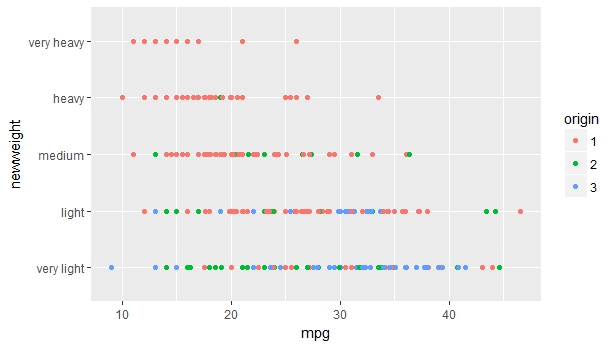
\includegraphics{conditionedweight.jpeg}
 
    \subsection{Discussion of Plot}
       Initially, I attempted to discretize the variables with 5 breakpoints, and got uneven bins.  Though there is some information contained in this type of distribution, that unevenness is not optimal for determining correlation or other tasks.  In this plot, there is a very clear relationship between mpg and weight, as well as between origin and those two variables.  Though there is a clear relationship, there are quite a few observations that fall outside of our relationship that I would address by adjusting the number of bins. \ldots   
\end{enumerate}

\end{homeworkProblem}


%%%%%%%%%%%%%%%%%%%%%%%%%%%%%%%%%

%PROBLEM 3
%%%%%%%%%%%%%%%%%%%%%%%%%%%%%%%%%%
\begin{homeworkProblem}
\subsection{Handling Missing Values  [50 pt]}

In this question, you will replace the missing data using different techniques. 


\begin{enumerate} 

\item How many entries are in the data set? There are 406 observations of 11 variables. $\ldots$
\rscript{sb6}{Sample R Script With Highlighting}
\item How many unknown or missing data are in the data set? There are two variables with missing values: mpg and horsepower, with 8 and 6 NA values, respectively. $\ldots$
\rscript{sb6}{Sample R Script With Highlighting}
\item Use \quotes{manyNAs} function to report the rows in the data that have certain number of unknowns ($nORp = 0.1$). There aren't any rows with more than 10 percent NA values, but there are 15 rows with 9 percent NA values. $\ldots$
\rscript{sb7}{Sample R Script With Highlighting}
\item Filling in the Unknowns with the Most Frequent Values:
\begin{enumerate}
\item  Replace missing values of variable \quotes{horsepower} and \quotes{mpg} variables using \quotes{centralImputation} function. Explain how this function fills in the unknown values.
\rscript{sb7}{Sample R Script With Highlighting}
\subsection{Discussion}
  The central imputation function fills in missing values with the statistic of centrality for our \quotes{mpg} column, here median as the column is a continuous variable.  After comparing the imputed values to values in complete rows, the imputed values don't seem to make sense, and may be higher than they should otherwise be. E.g. row 12, should have an mpg of between 17-19, but is imputed in my variable as 23, which is significantly higher than it should be and would cause issues for us down the road.  $\ldots$
\end{enumerate}
\item Filling in the Unknown Values by Exploring Correlations:
\begin{enumerate}
\item First, reload the original data that contains the missing data . Observe the correlations among the continuous variables (Variables 1,3,4,5,6) and report the correlation matrix (use symnum function). Discuss the results.
\rscript{sb8}{Sample R Script With Highlighting}
\subsection{Discussion and Correlation Matrix}
There are several interesting correlations between \quotes{weight}, \quotes{horsepower}, and \quotes{displacement} $\ldots$

\item What variable has the highest linear correlation with \quotes{horsepower} variable. Fit a linear model to fill in unknown values of \quotes{horsepower} via this variable. Report the new values of unknown data.
\rscript{sb9}{Sample R Script With Highlighting}
   \subsection{Results}
The displacement variable has the highest linear correlation with the horsepower variable.  The new values of missing data are between 46 and 48 mpg, which is in line with similar cases. $\ldots$
\end{enumerate}
\item Filling in the Unknown Values by Exploring Similarities between Cases:
\begin{enumerate}
\item  First, reload the original data that contains the missing data. Replace missing values of  the data set using \quotes{knnImputation()} function.  Explain how this function replaces the missing values (Pick, $k=5,\ meth$ = \quotes{median}).  The clean data obtained after using \quotes{knnImputation()} function will be the data set that must be used to answer  the rest of the problems.
\rscript{sb10}{Sample R Script With Highlighting}
\subsection{Discussion}
By specifying method as \quotes{median}, the knnImputation function fills in cases with NA values by using the median value of each continuous variable (or mode of categorical), as opposed to a weighted average. This function replaces the NA values in each row. $\ldots$
\end{enumerate}
\end{enumerate}
 
\end{homeworkProblem}

%%%%%%%%%%%%%%%%%%%%%%%%%%%%%%%%%

%PROBLEM 4
%%%%%%%%%%%%%%%%%%%%%%%%%%%%%%%%%%
\begin{homeworkProblem}

Use the clean data set from question $3.6.a$ to answer problem 4. Remove the last variable, car name, from the clean data before answering this question.
\subsection{Obtaining Predictive Models (Linear Regression and Regression Trees)  [50 pt]}

\begin{enumerate} 

\item  Simple linear regression: 
\begin{enumerate}
\item Obtain a linear model using variable \quotes{weight} to predict \quotes{mpg} variable. Use summary() function to explain the model and discuss output of summary() function, i.e., what does \quotes{Adjusted R-squared} show?, what are the coefficients?, etc. Is this a good model?

  \subsection{R Code}

\rscript{sb11}{Sample R Script With Highlighting}

\subsection{Discussion of Output of Summary() Function and Results}
      The residuals represent the difference between the observed values and the values the model predicted. The coefficients appear to be normally distributed, which at least indicates a consistent error.  The r-squared and adjusted r-squared indicate a relationship between our predictor and target variable. A value closer to 1 indicates that the relationship explains most of the variance. Here, we have an r-squared value of .39, which is not a very strong relationship. 

\item Plot the data points in a scatter plot (mpg vs. weight) and show the model from problem $4.a$ on this scatter plot?  Is the correlation between the variables positive or negative? There is a negative correlation of -.62 between the two variables.  This result makes sense, because as the mpg increases, the weight decreases, and vice versa. $\ldots$

\subsection{R Code}

\rscript{sb12}{Sample R Script With Highlighting}

   
\subsection{Figure}

 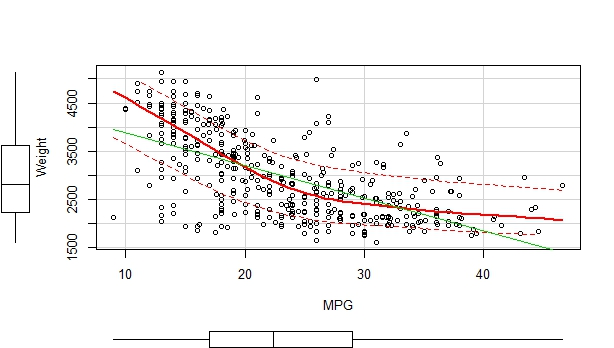
\includegraphics{p4scatterplot}

\end{enumerate}
\item  Multivariate linear regression:

\begin{enumerate}
\item Train a linear model that predicts variable \quotes{mpg} using all other variables (variables 2-8). Use summary() function to explain the model and discuss output of summary() function.

  \subsection{R Code}

\rscript{sb13}{Sample R Script With Highlighting}


\subsection{Discussion of Output of Summary() Function and Results}
       Our multi-variate linear model predicts mpg better than the \quotes{weight} variable alone by a significant amount. 

\item Use plot() function to understand performance of the model. Insert the four figures below and discuss the plots below that.

\subsection{Figure}

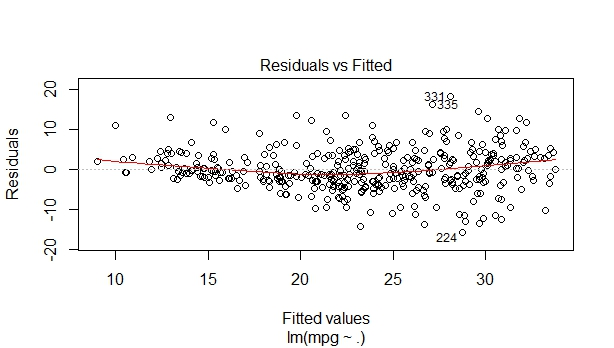
\includegraphics{residualsfitted}
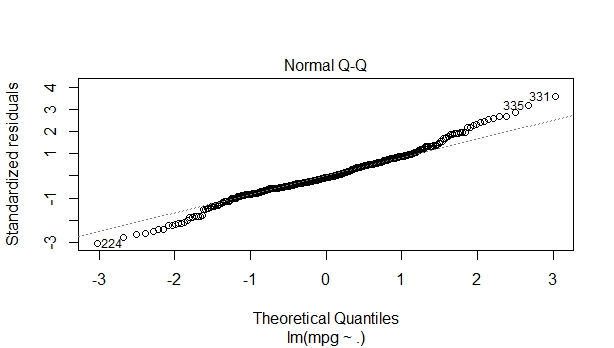
\includegraphics{p4normalqq}
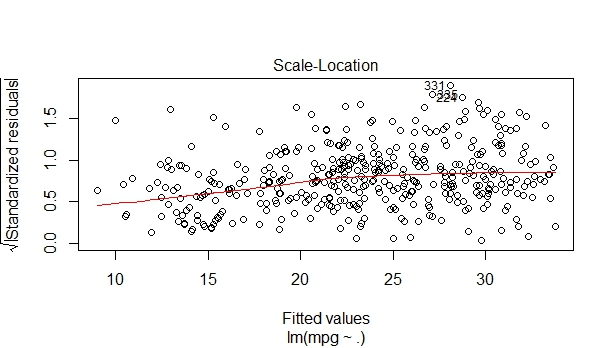
\includegraphics{p4scalelocation}
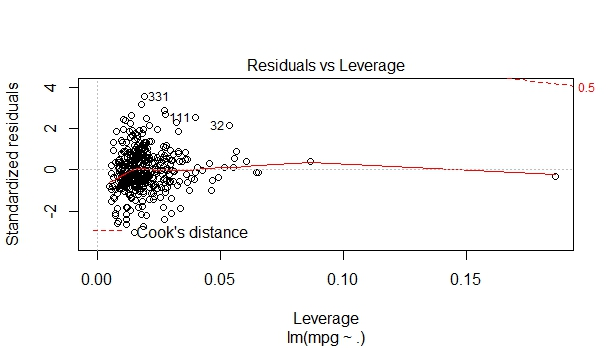
\includegraphics{cooks}
 
 
\subsection{Discussion of the Plots}
       The linear model may not have captured the non-linear relationship indicated by the first plot of Residuals vs. Fitted.  There is a slight negative parabolic curve to the data shown in the plot.  The Normal QQ plot of residual errors looks slightly skewed at the tails, though the overall distribution is close enough to normal.  The Scale-location or Spread Location plot looks close to normal, as the spread of residuals looks roughly the same near 10 as it does near 50, with the exception of a few outliers. Finally, in the last plot, there are no values outside of the dashed line, Cook's distance, that would materially alter the regression analysis, though there are several outliers.  In conclusion, though not optimal, this model does a mediocre to sufficient job of fitting the data. For the amount of effort we put into creating the model (one line of R plus some munging), the return on investment is decent.  

\item Find the variable that least contributes to the reduction of the fitting error of the model (use anova()). Then, use update() function to remove that variable from the model. How much of the variance is explained by this new model? Answer here \ldots 
\subsection{R Code}

\rscript{sb}{Sample R Script With Highlighting}


\item Use step() function to optimize the model obtained in question $4.a.$ and call this optimized model, \quotes{final.lm}
\subsection{R Code}

\rscript{sb14}{Sample R Script With Highlighting}
\end{enumerate}


\item  Regression Trees:
\begin{enumerate}
\item  Train a regression tree to predict \quotes{mpg} variable using all other variables (variables 2-8).  Visualize the tree. Call this model, \quotes{final.tree}.
  \subsection{R Code}

\rscript{sb15}{Sample R Script With Highlighting}


\subsection{Regression Tree Figure}
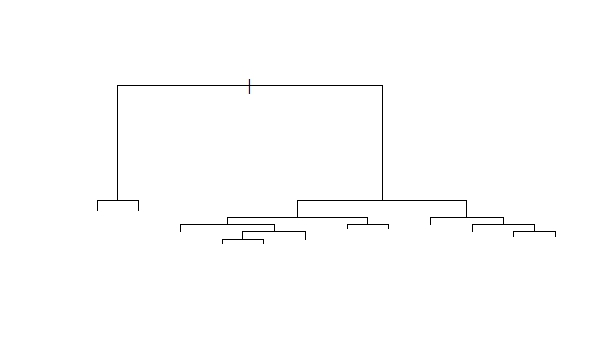
\includegraphics{finaltree}
 

\end{enumerate}

\end{enumerate}


\end{homeworkProblem}


%%%%%%%%%%%%%%%%%%%%%%%%%%%%%%%%%%

%PROBLEM 5
%%%%%%%%%%%%%%%%%%%%%%%%%%%%%%%%%%
\begin{homeworkProblem}
\subsection{Model Evaluation and Selection  [50 pt]}


Use the clean data set from question $3.6.a$ to answer problem 5. Remove the last variable, car name, from the clean data before answering this question. predict() function takes a model and  a test data and retrieves the corresponding model predictions.  In this question, you will use predict() function to compare final.lm and final.tree. Answer the questions below:

\begin{enumerate} 

\item  Calculate mean absolute error (MAE) for final.lm and final.tree. Which one is better? The tree prediction model has an MAE of 3.91 vs. 4.48 for the linear model.$\ldots$

  \subsection{R Code}

\rscript{sb16}{Sample R Script With Highlighting}

\item  Calculate mean squared error (MSE ) for final.lm and final.tree. Which one is better? Again, the tree model wins with a lower MSE of 2.57 vs. 3.48 for the linear model. $\ldots$

  \subsection{R Code}

\rscript{sb17}{Sample R Script With Highlighting}

\item  Calculate normalized mean squared error (NMSE ) for final.lm and final.tree. Which one is better? Answer here. The tree model wins again - 2.42 vs. 5.75 NMSE $\ldots$

  \subsection{R Code}

\rscript{sb18}{Sample R Script With Highlighting}

 \item  Observe the errors for final.lm and final.tree via scatter plots.  See figure 4.11, texbook, page 227. Discuss the plots, i.e., did the models perform well? 

\subsection{Error Scatter Plots}

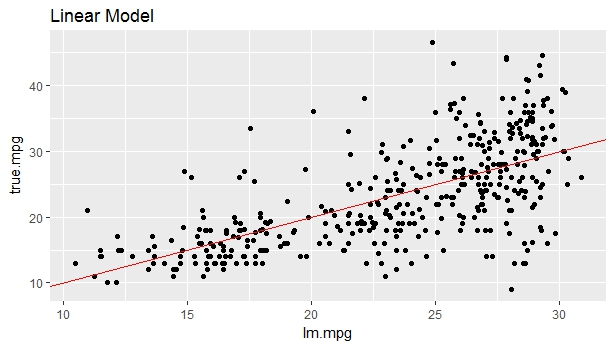
\includegraphics{p5lmscatter}
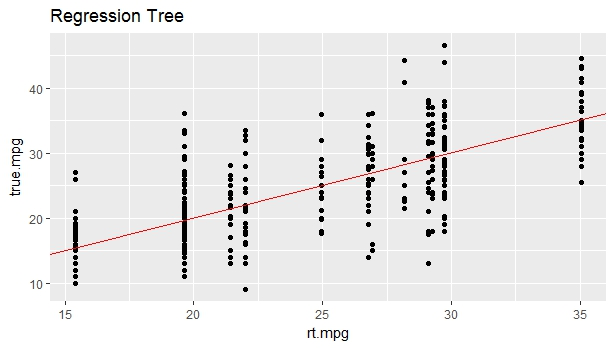
\includegraphics{p5treescatter}

  \subsection{R Code}

\rscript{sb19}{Sample R Script With Highlighting}


  \subsection{Discussion of the Error Plots}
        The error plots appear to confirm what we already know, which is that the regression tree performed better.  The values were less spread out over the regression tree plot, but both models only fit the data with mediocre results. The linear model was more accurate at predicting lower-valued mpg values, though that was likely because 1) there were fewer values, and 2) the other variables were likely less distributed for cars (observations) with lower mpgs (target variable.)  \ldots 

\item Cross Validation is a technique to measure performance of  models over unseen data. In this question, use performanceEstimation() function in R to make use of cross validation technique and compare several models. Take the performanceEstimation() code  from the textbook, page 228 and edit it for your data -- Fit one linear and three regression tree models with the given parameters.  Only tune the parameters of the \quotes{EstimationsTask as follows}:
 
 \begin{itemize}
 \item  EstimationsTask: metric= \quotes{mse} ,  method=CV(nReps=3,nFolds=5)
 \end{itemize}
 
 
 \subsection{R Code}

\rscript{sb}{Sample R Script With Highlighting}

 Answer the question below:

\begin{enumerate}

\item This function (according to the documentation) provides bootstrap estimates of the performance of a predictive task, e.g. our linear model or regression tree.  

  \subsection{Discussion of performanceEstimation() Function }
  Answer here \ldots

\item Compare the models? Which model performed best? The final model that performed the best appears to be the linear model with 5 reps of 10 folds. $\ldots$


\end{enumerate}

\end{enumerate}


\end{homeworkProblem}

%%%%%%%%%%%%%%%%%%%%%%%%%%%%%%%%%%

\end{document}